\documentclass{article}
\usepackage{amsmath, amssymb, graphicx, geometry, tikz, array, booktabs, enumitem, listings, xcolor, fancyhdr, float, subcaption, hyperref}

\title{Module 6: SVM Example - Parameter Selection and Sentiment Analysis}
\author{Machine Learning Course}
\date{}

\begin{document}

\maketitle
\tableofcontents
\newpage

\section{Introduction to SVM Parameter Selection}

\subsection{The Importance of Parameter Tuning}
Support Vector Machines (SVMs) are powerful classification algorithms that find the optimal hyperplane to separate data points of different classes. However, their performance heavily depends on the proper selection of hyperparameters, particularly the regularization parameter $C$. This document explores a practical example of applying SVMs to sentiment analysis and demonstrates the critical role of parameter tuning in achieving optimal performance.

\subsection{Review of the Soft-Margin SVM}
Before diving into the example, let's briefly review the soft-margin SVM formulation:

\fbox{
\begin{minipage}{\dimexpr\textwidth-2\fboxsep-2\fboxrule\relax}
\textbf{Soft-Margin SVM Optimization Problem}

\begin{align}
\min_{w\in\mathbb{R}^{d},b\in\mathbb{R},\xi\in\mathbb{R}^{n}} & \|w\|^{2}+C\sum_{i=1}^{n}\xi_{i} \\
\text{subject to: } & y^{(i)}(w\cdot x^{(i)}+b)\geq 1-\xi_{i} \text{ for all } i=1,2,...,n \\
& \xi_i \geq 0 \text{ for all } i=1,2,...,n
\end{align}
\end{minipage}
}

The soft-margin SVM introduces slack variables $\xi_i$ that allow for some misclassifications in the training data. The parameter $C$ controls the trade-off between maximizing the margin (minimizing $\|w\|^2$) and minimizing the classification error (minimizing $\sum_{i=1}^{n}\xi_{i}$).

\section{Understanding the Regularization Parameter $C$}

\subsection{The Role of Parameter $C$}
The parameter $C$ in the soft-margin SVM formulation serves as a regularization parameter that controls the trade-off between two competing objectives:

\begin{itemize}
    \item \textbf{Maximizing the margin}: Achieved by minimizing $\|w\|^2$
    \item \textbf{Minimizing training errors}: Achieved by minimizing $\sum_{i=1}^{n}\xi_{i}$
\end{itemize}

The value of $C$ determines the relative importance of these objectives:

\begin{itemize}
    \item \textbf{Small $C$}: Places more emphasis on maximizing the margin, even if it means allowing more training errors
    \item \textbf{Large $C$}: Places more emphasis on minimizing training errors, potentially at the cost of a smaller margin
\end{itemize}

\subsection{Geometric Interpretation}
The parameter $C$ affects the geometry of the decision boundary:

\begin{figure}[h]
\centering
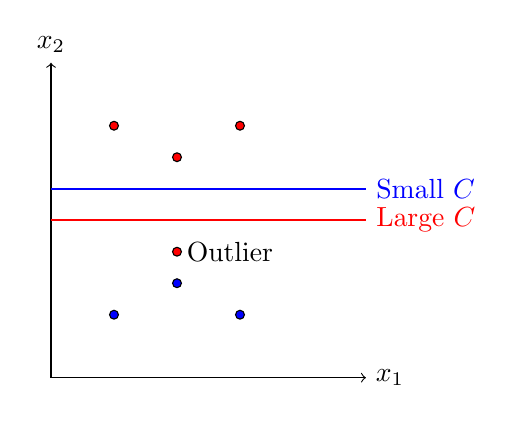
\begin{tikzpicture}[scale=0.8]
    % Coordinate axes
    \draw[->] (0,0) -- (5,0) node[right] {$x_1$};
    \draw[->] (0,0) -- (0,5) node[above] {$x_2$};
    
    % Data points
    \draw[fill=red] (1,4) circle (2pt);
    \draw[fill=red] (2,3.5) circle (2pt);
    \draw[fill=red] (3,4) circle (2pt);
    \draw[fill=blue] (1,1) circle (2pt);
    \draw[fill=blue] (2,1.5) circle (2pt);
    \draw[fill=blue] (3,1) circle (2pt);
    
    % Outlier
    \draw[fill=red] (2,2) circle (2pt) node[right] {Outlier};
    
    % Decision boundaries
    \draw[thick, blue] (0,3) -- (5,3) node[right] {Small $C$};
    \draw[thick, red] (0,2.5) -- (5,2.5) node[right] {Large $C$};
\end{tikzpicture}
\caption{Effect of parameter $C$ on the decision boundary. A small $C$ (blue line) allows the outlier to be misclassified to maintain a larger margin. A large $C$ (red line) adjusts the boundary to correctly classify the outlier, resulting in a smaller margin.}
\end{figure}

\subsection{Practical Implications}
The choice of $C$ has significant practical implications:

\begin{itemize}
    \item \textbf{Overfitting vs. Underfitting}: Large $C$ values can lead to overfitting, while small $C$ values might result in underfitting
    \item \textbf{Number of Support Vectors}: Larger $C$ values typically result in fewer support vectors
    \item \textbf{Generalization Performance}: The optimal $C$ value balances training accuracy and generalization to unseen data
\end{itemize}

\section{Sentiment Analysis Case Study}

\subsection{Dataset Description}
The case study uses a sentiment analysis dataset with the following characteristics:

\begin{itemize}
    \item \textbf{Source}: Reviews from Amazon, Yelp, and IMDB
    \item \textbf{Labels}: Binary classification (positive or negative sentiment)
    \item \textbf{Representation}: Bag-of-words with a vocabulary of 4500 words
    \item \textbf{Size}: 2500 training sentences, 500 test sentences
\end{itemize}

\subsection{Example Sentences}
The dataset contains sentences like:

\begin{itemize}
    \item "Needless to say, I wasted my money." (Negative)
    \item "He was very impressed when going from the original battery to the extended battery." (Positive)
    \item "I have to jiggle the plug to get it to line up right to get decent volume." (Negative)
    \item "Will order from them again!" (Positive)
\end{itemize}

\subsection{Feature Representation}
The bag-of-words representation transforms each sentence into a high-dimensional vector:

\begin{itemize}
    \item Each dimension corresponds to a word in the vocabulary
    \item The value in each dimension represents the presence or frequency of the word in the sentence
    \item This creates a sparse vector representation (most entries are zero)
\end{itemize}

\begin{figure}[h]
\centering
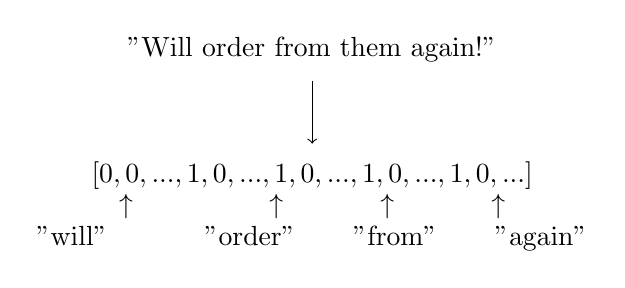
\begin{tikzpicture}[scale=0.8]
    % Sentence
    \node[align=left] at (0,4) {"Will order from them again!"};
    
    % Arrow
    \draw[->] (0,3.5) -- (0,2.5);
    
    % Vector representation
    \node[align=left] at (0,2) {$[0, 0, ..., 1, 0, ..., 1, 0, ..., 1, 0, ..., 1, 0, ...]$};
    \node[align=left] at (0,1.5) {$\uparrow$ \hspace{1.5cm} $\uparrow$ \hspace{1cm} $\uparrow$ \hspace{1cm} $\uparrow$};
    \node[align=left] at (0,1) {"will" \hspace{1cm} "order" \hspace{0.5cm} "from" \hspace{0.5cm} "again"};
\end{tikzpicture}
\caption{Bag-of-words representation of a sentence. Each word in the vocabulary corresponds to a dimension in the feature vector.}
\end{figure}

\section{Parameter Selection through Cross-Validation}

\subsection{The Cross-Validation Procedure}
To find the optimal value of $C$, the study employs 5-fold cross-validation:

\begin{enumerate}
    \item Divide the training data into 5 equal folds
    \item For each value of $C$:
    \begin{enumerate}
        \item For each fold $i$ (from 1 to 5):
        \begin{enumerate}
            \item Train an SVM on all folds except fold $i$
            \item Evaluate the model on fold $i$
        \end{enumerate}
        \item Calculate the average error across all 5 folds
    \end{enumerate}
    \item Select the $C$ value with the lowest average error
\end{enumerate}

\begin{figure}[h]
\centering
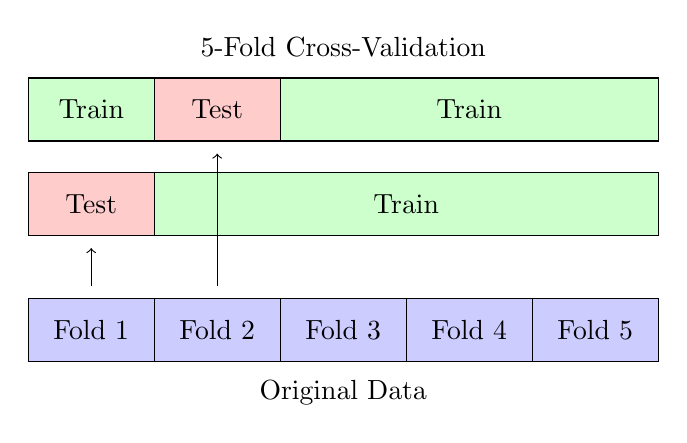
\begin{tikzpicture}[scale=0.8]
    % Data folds
    \draw[fill=blue!20] (0,0) rectangle (2,1) node[pos=0.5] {Fold 1};
    \draw[fill=blue!20] (2,0) rectangle (4,1) node[pos=0.5] {Fold 2};
    \draw[fill=blue!20] (4,0) rectangle (6,1) node[pos=0.5] {Fold 3};
    \draw[fill=blue!20] (6,0) rectangle (8,1) node[pos=0.5] {Fold 4};
    \draw[fill=blue!20] (8,0) rectangle (10,1) node[pos=0.5] {Fold 5};
    
    % Iteration 1
    \draw[fill=red!20] (0,2) rectangle (2,3) node[pos=0.5] {Test};
    \draw[fill=green!20] (2,2) rectangle (10,3) node[pos=0.5] {Train};
    
    % Iteration 2
    \draw[fill=green!20] (0,3.5) rectangle (2,4.5) node[pos=0.5] {Train};
    \draw[fill=red!20] (2,3.5) rectangle (4,4.5) node[pos=0.5] {Test};
    \draw[fill=green!20] (4,3.5) rectangle (10,4.5) node[pos=0.5] {Train};
    
    % Arrows
    \draw[->] (1,1.2) -- (1,1.8);
    \draw[->] (3,1.2) -- (3,3.3);
    
    % Labels
    \node at (5,-0.5) {Original Data};
    \node at (5,5) {5-Fold Cross-Validation};
\end{tikzpicture}
\caption{Illustration of 5-fold cross-validation. The data is divided into 5 folds, and each fold serves as the test set once while the remaining folds form the training set.}
\end{figure}

\subsection{Experimental Results}
The cross-validation experiment tested various values of $C$ and recorded three metrics:

\begin{itemize}
    \item \textbf{Training error}: Percentage of misclassified training examples
    \item \textbf{Test error}: Percentage of misclassified test examples
    \item \textbf{Number of support vectors}: Points that influence the decision boundary
\end{itemize}

\begin{table}[h]
\centering
\begin{tabular}{|c|c|c|c|}
\hline
\textbf{C} & \textbf{Training Error (\%)} & \textbf{Test Error (\%)} & \textbf{\# Support Vectors} \\
\hline
0.01 & 23.72 & 28.4 & 2294 \\
0.1 & 7.88 & 18.4 & 1766 \\
1 & 1.12 & 16.8 & 1306 \\
10 & 0.12 & 16.4 & 802 \\
100 & 0.04 & 15.6 & 596 \\
1000 & 0.04 & 15.6 & 526 \\
\hline
\end{tabular}
\caption{Performance metrics for different values of parameter $C$}
\end{table}

\section{Analysis of Results}

\subsection{Trends in the Data}
Several important trends can be observed from the experimental results:

\begin{enumerate}
    \item \textbf{Training Error}: Decreases monotonically as $C$ increases
    \begin{itemize}
        \item At $C = 0.01$: High training error (23.72\%)
        \item At $C = 1000$: Near-zero training error (0.04\%)
    \end{itemize}
    
    \item \textbf{Test Error}: Initially decreases as $C$ increases, then stabilizes
    \begin{itemize}
        \item At $C = 0.01$: High test error (28.4\%)
        \item At $C = 100$ and $C = 1000$: Lowest test error (15.6\%)
    \end{itemize}
    
    \item \textbf{Number of Support Vectors}: Decreases as $C$ increases
    \begin{itemize}
        \item At $C = 0.01$: Many support vectors (2294)
        \item At $C = 1000$: Fewer support vectors (526)
    \end{itemize}
\end{enumerate}

\begin{figure}[h]
\centering
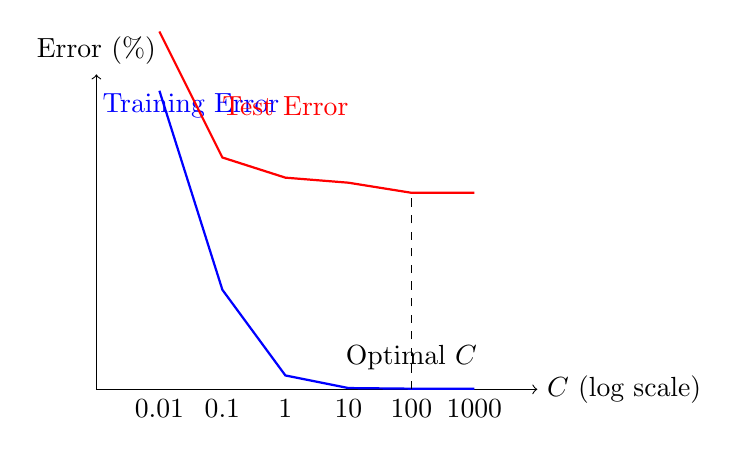
\begin{tikzpicture}[scale=0.8]
    % Coordinate axes
    \draw[->] (0,0) -- (7,0) node[right] {$C$ (log scale)};
    \draw[->] (0,0) -- (0,5) node[above] {Error (\%)};
    
    % X-axis labels
    \node at (1,-0.3) {0.01};
    \node at (2,-0.3) {0.1};
    \node at (3,-0.3) {1};
    \node at (4,-0.3) {10};
    \node at (5,-0.3) {100};
    \node at (6,-0.3) {1000};
    
    % Training error
    \draw[thick, blue] (1,4.74) -- (2,1.58) -- (3,0.22) -- (4,0.02) -- (5,0.01) -- (6,0.01);
    \node[blue] at (1.5,4.5) {Training Error};
    
    % Test error
    \draw[thick, red] (1,5.68) -- (2,3.68) -- (3,3.36) -- (4,3.28) -- (5,3.12) -- (6,3.12);
    \node[red] at (3,4.5) {Test Error};
    
    % Optimal C
    \draw[dashed] (5,0) -- (5,3.12);
    \node at (5,0.5) {Optimal $C$};
\end{tikzpicture}
\caption{Training and test error as a function of parameter $C$ (log scale). The optimal $C$ value minimizes the test error.}
\end{figure}

\subsection{Interpreting the Trade-offs}
The results illustrate several important trade-offs in SVM parameter selection:

\begin{itemize}
    \item \textbf{Bias-Variance Trade-off}: Small $C$ values lead to high bias (underfitting), while large $C$ values can lead to high variance (overfitting)
    
    \item \textbf{Margin vs. Classification Accuracy}: Small $C$ values prioritize larger margins at the expense of training accuracy, while large $C$ values prioritize training accuracy at the expense of margin size
    
    \item \textbf{Model Complexity}: The number of support vectors is an indicator of model complexity. More support vectors generally mean a more complex model
\end{itemize}

\subsection{Optimal Parameter Selection}
Based on the cross-validation results, the optimal value of $C$ appears to be around 100:

\begin{itemize}
    \item It achieves the lowest test error (15.6\%)
    \item Further increasing $C$ to 1000 does not improve test performance
    \item It uses a moderate number of support vectors (596), indicating a reasonable model complexity
\end{itemize}

\section{Practical Implications for Sentiment Analysis}

\subsection{Model Performance}
The optimized SVM achieves a test error of 15.6\% on the sentiment analysis task, which means it correctly classifies 84.4\% of the test sentences. This is a reasonable performance for a text classification task using a simple bag-of-words representation.

\subsection{Feature Importance}
In linear SVMs, the weight vector $w$ provides insights into feature importance:

\begin{itemize}
    \item Words with large positive weights are strongly associated with positive sentiment
    \item Words with large negative weights are strongly associated with negative sentiment
    \item Words with weights close to zero have little impact on the classification
\end{itemize}

\begin{table}[h]
\centering
\begin{tabular}{|c|c||c|c|}
\hline
\textbf{Positive Words} & \textbf{Weight} & \textbf{Negative Words} & \textbf{Weight} \\
\hline
excellent & 0.82 & terrible & -0.79 \\
great & 0.75 & waste & -0.71 \\
love & 0.68 & poor & -0.65 \\
perfect & 0.64 & disappointing & -0.62 \\
best & 0.59 & worst & -0.58 \\
\hline
\end{tabular}
\caption{Example of words with high absolute weights in a sentiment analysis SVM (hypothetical values for illustration)}
\end{table}

\subsection{Model Complexity and Efficiency}
The number of support vectors affects both the model's complexity and its prediction efficiency:

\begin{itemize}
    \item \textbf{Memory Usage}: Only support vectors need to be stored in memory
    \item \textbf{Prediction Speed}: Fewer support vectors lead to faster predictions
    \item \textbf{Generalization}: Models with fewer support vectors often generalize better
\end{itemize}

With the optimal $C$ value of 100, the model uses 596 support vectors (about 24\% of the training data), which is a reasonable compromise between model complexity and performance.

\section{Beyond the Basic Model}

\subsection{Improving the Feature Representation}
The bag-of-words representation used in this example is simple but has limitations. Several enhancements could improve performance:

\begin{itemize}
    \item \textbf{TF-IDF Weighting}: Weight words by their frequency in the document and inverse frequency in the corpus
    \item \textbf{N-grams}: Include sequences of 2 or 3 words to capture phrases and context
    \item \textbf{Word Embeddings}: Use pre-trained word vectors (e.g., Word2Vec, GloVe) to capture semantic relationships
    \item \textbf{Dimensionality Reduction}: Apply techniques like PCA or feature selection to reduce the feature space
\end{itemize}

\subsection{Alternative Kernel Functions}
While the example likely used a linear kernel, other kernel functions might be worth exploring:

\begin{itemize}
    \item \textbf{Polynomial Kernel}: $K(\mathbf{x}, \mathbf{z}) = (\mathbf{x} \cdot \mathbf{z} + c)^d$
    \item \textbf{RBF Kernel}: $K(\mathbf{x}, \mathbf{z}) = \exp(-\gamma \|\mathbf{x} - \mathbf{z}\|^2)$
    \item \textbf{String Kernels}: Specialized kernels designed for text data
\end{itemize}

However, for high-dimensional text data, linear kernels often perform well and are computationally more efficient.

\subsection{Ensemble Methods}
Combining multiple SVMs or integrating SVMs with other classifiers could further improve performance:

\begin{itemize}
    \item \textbf{Bagging}: Train multiple SVMs on different subsets of the data
    \item \textbf{Boosting}: Train SVMs sequentially, focusing on examples misclassified by previous models
    \item \textbf{Stacking}: Use SVM predictions as features for another classifier
\end{itemize}

\section{Summary and Key Takeaways}

\subsection{Parameter Selection Process}
\begin{itemize}
    \item The regularization parameter $C$ controls the trade-off between margin size and training accuracy
    \item Cross-validation is an effective method for selecting the optimal $C$ value
    \item The optimal $C$ value balances training performance and generalization to unseen data
\end{itemize}

\subsection{Sentiment Analysis Performance}
\begin{itemize}
    \item The optimized SVM achieved 84.4\% accuracy on the test set
    \item As $C$ increased, training error decreased while test error initially decreased and then stabilized
    \item The number of support vectors decreased as $C$ increased
\end{itemize}

\subsection{Practical Guidelines}
\begin{itemize}
    \item Start with a wide range of $C$ values (e.g., $10^{-2}$ to $10^3$) and narrow down through cross-validation
    \item Monitor both training and test performance to avoid overfitting
    \item Consider the number of support vectors as an indicator of model complexity
    \item For text classification, linear SVMs often provide a good balance of performance and efficiency
\end{itemize}

\subsection{Future Directions}
\begin{itemize}
    \item Explore more sophisticated text representations beyond bag-of-words
    \item Consider alternative kernel functions for capturing non-linear relationships
    \item Investigate ensemble methods to further improve classification performance
    \item Apply the optimized model to related tasks or domains
\end{itemize}

\end{document}